\section*{Tarea 1 (P23.2)}

Sabiendo que el número atómico de la plata es $47$, se tienen esa cantidad de electrones. Entonces, utilizando el número de avogadro\footnote{Es el factor de proporcionalidad que relaciona el número de partículas en una muestra con la cantidad de sustancia de la misma.} y con un poco de aritmética se llega a
	$$ N = \qty(\frac{10g}{107.87g/\text{mol}}) \qty(6.022\times 10^{23} \text{atomos}/\text{mol}) \qty(47 \text{electrones}/\text{atomo}) = 2.62\times 10^{24} \text{electrones}. $$
	
Ahora, encontramos el número de electrones en $1mC$
	$$ \frac{Q}{e} = \frac{1mC}{1.6\times 10^{15}} = 6.24\times 10^{15} \text{electrones}, $$

que con un poco de aritmética, se encuentra que hay $2.38$ electrones agregados por cada $10^9$ existentes.








\section*{Tarea 2 (P23.7)}

Dado el sistema, se tiene el siguiente diagrama con las respectivas fuerzas actuando sobre $q_2$.
\begin{center}
	


\tikzset{every picture/.style={line width=0.75pt}} %set default line width to 0.75pt        

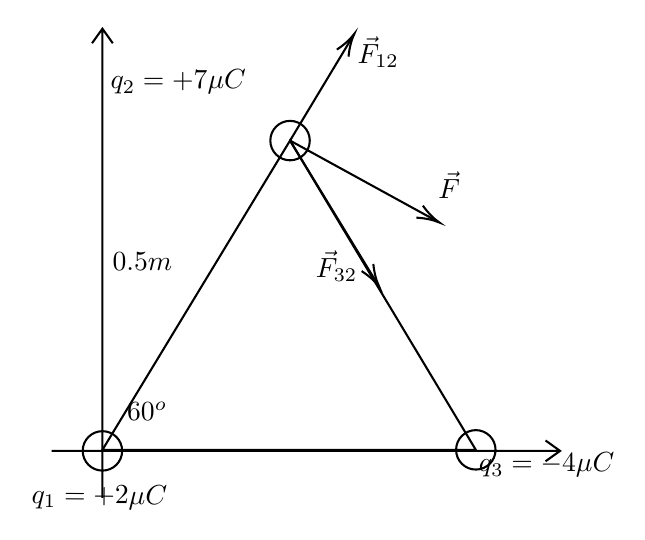
\begin{tikzpicture}[x=0.75pt,y=0.75pt,yscale=-1,xscale=1]
%uncomment if require: \path (0,300); %set diagram left start at 0, and has height of 300

%Shape: Triangle [id:dp9976522048032088] 
\draw   (267,67.5) -- (356.5,216.5) -- (176.6,216.5) -- cycle ;
%Shape: Circle [id:dp5539049513903027] 
\draw   (167.1,217) .. controls (167.1,211.75) and (171.35,207.5) .. (176.6,207.5) .. controls (181.85,207.5) and (186.1,211.75) .. (186.1,217) .. controls (186.1,222.25) and (181.85,226.5) .. (176.6,226.5) .. controls (171.35,226.5) and (167.1,222.25) .. (167.1,217) -- cycle ;
%Shape: Circle [id:dp03557687797226117] 
\draw   (347,216.5) .. controls (347,211.25) and (351.25,207) .. (356.5,207) .. controls (361.75,207) and (366,211.25) .. (366,216.5) .. controls (366,221.75) and (361.75,226) .. (356.5,226) .. controls (351.25,226) and (347,221.75) .. (347,216.5) -- cycle ;
%Shape: Axis 2D [id:dp35701988623397174] 
\draw  (152.1,217) -- (397.1,217)(176.6,13.6) -- (176.6,239.6) (390.1,212) -- (397.1,217) -- (390.1,222) (171.6,20.6) -- (176.6,13.6) -- (181.6,20.6)  ;
%Shape: Circle [id:dp21574096627013728] 
\draw   (257.5,67.5) .. controls (257.5,62.25) and (261.75,58) .. (267,58) .. controls (272.25,58) and (276.5,62.25) .. (276.5,67.5) .. controls (276.5,72.75) and (272.25,77) .. (267,77) .. controls (261.75,77) and (257.5,72.75) .. (257.5,67.5) -- cycle ;
%Straight Lines [id:da743332007005598] 
\draw    (267,67.5) -- (308.96,136.29) ;
\draw [shift={(310,138)}, rotate = 238.62] [color={rgb, 255:red, 0; green, 0; blue, 0 }  ][line width=0.75]    (10.93,-3.29) .. controls (6.95,-1.4) and (3.31,-0.3) .. (0,0) .. controls (3.31,0.3) and (6.95,1.4) .. (10.93,3.29)   ;
%Straight Lines [id:da4895454589919841] 
\draw    (267,67.5) -- (337.25,106.04) ;
\draw [shift={(339,107)}, rotate = 208.75] [color={rgb, 255:red, 0; green, 0; blue, 0 }  ][line width=0.75]    (10.93,-3.29) .. controls (6.95,-1.4) and (3.31,-0.3) .. (0,0) .. controls (3.31,0.3) and (6.95,1.4) .. (10.93,3.29)   ;

%Straight Lines [id:da8197536808983341] 
\draw    (267,67.5) -- (296.97,17.71) ;
\draw [shift={(298,16)}, rotate = 121.05] [color={rgb, 255:red, 0; green, 0; blue, 0 }  ][line width=0.75]    (10.93,-3.29) .. controls (6.95,-1.4) and (3.31,-0.3) .. (0,0) .. controls (3.31,0.3) and (6.95,1.4) .. (10.93,3.29)   ;

% Text Node
\draw (179,32) node [anchor=north west][inner sep=0.75pt]    {$q_{2} =+7\mu C$};
% Text Node
\draw (298,16) node [anchor=north west][inner sep=0.75pt]    {$\vec{F}_{12}$};
% Text Node
\draw (337,81) node [anchor=north west][inner sep=0.75pt]    {$\vec{F}$};
% Text Node
\draw (278,119) node [anchor=north west][inner sep=0.75pt]    {$\vec{F}_{32}$};
% Text Node
\draw (187,192) node [anchor=north west][inner sep=0.75pt]    {$60^{o}$};
% Text Node
\draw (180,120) node [anchor=north west][inner sep=0.75pt]    {$0.5m$};
% Text Node
\draw (356.5,216.5) node [anchor=north west][inner sep=0.75pt]    {$q_{3} =-4\mu C$};
% Text Node
\draw (141.09,231.66) node [anchor=north west][inner sep=0.75pt]  [rotate=-0.42]  {$q_{1} =+2\mu C$};


\end{tikzpicture}

\end{center}

Con el diagrama mostrado, se tienen las dos fuerzas actuando sobre $q_2$
	$$ \vec{F} _{12} = \frac{1}{4\pi \varepsilon _o} \frac{\abs{q_1 q_2}}{r^2} \qty(\cos{60} \vx + \sin{60} \vy), $$
	$$ \vec{F} _{32} = \frac{1}{4\pi \varepsilon _o} \frac{\abs{q_2 q_3}}{r^2} \qty(\cos{60} \vx - \sin{60} \vy). $$
Sumando ambas fuerzas y valuando valores:
	$$ \vec{F} = 0.755 N \vx - 0.436N\vy , $$
o $\abs{F} = 0.872N$ a $\theta = -30^o$.











\section*{Tarea 3 (P23.39)}

La dirección del campo eléctrico será la misma dirección que el movimiento del haz de elecrones. Para la magnitud se tiene, por teorema trabajo-energía
	$$ W_{neto} = \Delta K, $$
	$$ -\underbrace{F}_{eE} d = 0 - K, $$
	$$ \therefore \quad E = \frac{K}{ed}. $$











\section*{Tarea 4 (P24.43)}

El área de un casquete esférico de la siguiente forma
	\begin{figure}[H]
		\centering
		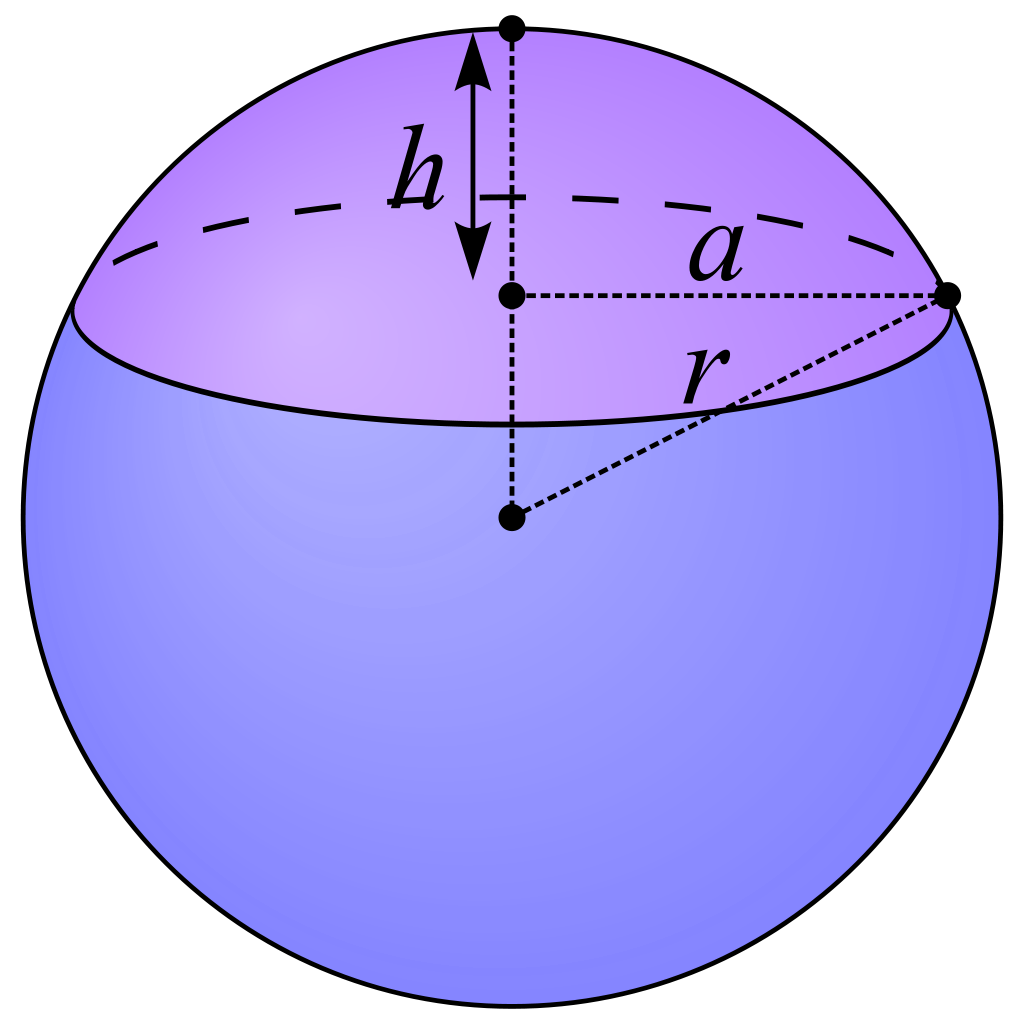
\includegraphics[scale=0.1]{./img/casquete.png}
		\caption{Casquete esférico.}
		\label{casq}
	\end{figure}
es: $ A = \pi (a^2 + h^2) \quad \Rightarrow \quad A = 2\pi r^2 \qty(1-\cos{\theta}) $. Con esto y teniendo el campo eléctrico de una carga puntual
	$$ \Phi _E = \qty[2\pi r^2 (1-\cos{\theta})]\qty[\frac{Q}{4\pi \varepsilon _o r^2}], $$
	$$ \Phi _E = \frac{Q}{2\varepsilon _o} (1 - \cos{\theta}). $$
Para $\theta = 90^o$:
	$$ \Phi _E (\theta = 90^o) = \frac{Q}{2\varepsilon _o} $$
flujo en una semiesfera. \\
Para $\theta = 180^o$:
	$$ \Phi _E (\theta = 180^o) = \frac{Q}{\varepsilon _o} $$
flujo en una esfera completa, el caso "base" de la ley de Gauss.











\section*{Tarea 5 (P25.39)}

\begin{enumerate}[a)]
	\item Como se trata de un conductor, el campo dentro de él es cero. Mientras que el voltaje tiene un valor de
		$$ V = \frac{q}{4\pi \varepsilon _o r} = 1.67\times 10^{6} V. $$
	\item Fuera de la esfera el campo se comporta como el de una carga puntual, por ende
		$$ E(0.2) = 5.8\times 10^{6} N/C, $$
		$$ V(0.2) = 1.168\times 10^{6} V. $$
	\item Al igual que el anterior inciso, es equivalente a una carga puntual.
		$$ E(0.14) = 11.9\times 10^{6} N/C, $$
		$$ V(0.14) = 1.67\times 10^{6} V. $$
\end{enumerate}











\section*{Tarea 6 (P25.31)}

Dado que $\vec{E} = -\grad{V}$, entonces
	$$ \vec{E} = -\qty(\pdv{V}{x} \vx + \pdv{V}{y} \vy + \pdv{V}{z} \vz) = \qty(6xy - 5) \vx + \qty(3x^2 - 2z^2) \vy - \qty(4yz) \vz , $$
valuando para $(1,0,-2)$, el valor del campo en dicho punto es
	$$ \boxed{ E(1,0,-2) = -5(\vx + \vy). } $$
	
Entonces
	$$ \boxed{ \abs{\vec{E}} = 5\sqrt{2} N/C .} $$








\section*{Tarea 7 (P26.1)}


Tomando la definición de capacitancia
	$$ C = \frac{Q}{V_{AB}}, $$
se tiene
	\begin{enumerate}[a)]
		\item Para $C = 4\mu F$ y $12V$, se tiene $48\mu C$.
		\item Para $C = 4\mu F$ y $1.5V$, se tiene $6\mu C$.
	\end{enumerate}







\section*{Tarea 8 (P28.2)}


\begin{enumerate}[a)]
	\item Calculamos la corriente $I = \frac{\varepsilon}{R + r}$ y, con esto, la diferencia de potencial.
		$$ \boxed{ \Delta V = IR = 12.4V } $$
	\item Se tiene que $I_{\text{bateria}} = I_{\text{luces}} + I_{\text{carro}}$, por la batería $\varepsilon = I_{\text{bateria}} r + I_{\text{luces}} R$, sustituyendo la corriente de la batería encontramos la corriente por las luces $I_{\text{luces}} = 1.93A$. Con esto, encontramos la diferencia de potencial
		$$ \boxed{\Delta V = 1.93A*5\Omega = 9.65V .} $$
\end{enumerate}










\section*{Tarea 9 (P27.27)}

Dado que la resistencia no cambia, se tiene la razón entre la potencia a $120V$ y $140V$ es de
	$$ \frac{\mathcal{P}}{\mathcal{P_o}} = \frac{V^2 /R}{V_o ^2 /R} = \qty(\frac{140}{120})^2 = 1.361. $$
Por lo que, el incremento es
	$$ \Delta \% = \qty(\frac{P - P_o}{P_o}) \boxed{ = 36.1\% .} $$







\section*{Tarea 10 (P28.13)}


La resistencia \textbf{disminuye}. La resistencia con el switch abierto es:
	$$ R + \frac{1}{\frac{1}{90 + 10} + \frac{1}{90 + 10}} = R + 50\Omega . $$
	Mientras que la nueva resistencia equivalente se calcula por malla
	$$ R + \frac{1}{\frac{1}{90} + \frac{1}{10}} + \frac{1}{\frac{1}{90} + \frac{1}{10}} = R + 18\Omega . $$

Si el factor es de $2$, el valor de la resistencia es de $R = 14\Omega$.









\section*{Tarea 11 (P28.55)}

\begin{enumerate}[a)]
	\item Encontramos la resistencia de cada foco, que es la misma, por ende
			$$ R = \frac{\Delta V ^2}{\mathcal{P}} = 240 \Omega . $$
		Con esto, se encuentra la resistencia equivalente
			$$ R_e = R + \qty(\frac{1}{\frac{1}{R} + \frac{1}{R}}) = 60\Omega , $$
		entonces, $\mathcal{P} = \flatfrac{120^2}{360} = \boxed{40W.}$
	\item Ahora, para el foco $1$, se tiene que la corriente es $I = \sqrt{\flatfrac{\mathcal{P}}{R_e}} = 1/3 A$, entonces $\Delta V_1 = I R = \boxed{80V}$. Para el foco $2$ y $3$ se tiene el mismo voltaje en ambos, por lo que utilizando ese arreglo en conjunto se tiene
		$$ \Delta V_{23} = \qty(\frac{1}{3} A) \frac{1}{\frac{1}{R} + \frac{1}{R}} = \boxed{40V.} $$
\end{enumerate}















\section*{Tarea 12 (P30.11)}

Se sabe que para un conductor recto el campo es
	$$ B = \frac{\mu _o I}{2\pi r}. $$
\begin{description}
	\item[A:] Por la regla de la mano derecha se tiene el siguiente valor para el campo en $A$
		$$ B_A = B_1 \cos{\pi /4} + B_2 \cos{\pi /4} + B_3, $$
			con $B_1 = B_2$
				$$ B_A = 2\qty(\frac{\mu _o I}{2\pi a\sqrt{2}}) \cos{\pi /4} + \frac{\mu _o I}{2\pi (3a)} = \boxed{ 53.3\mu T \, \downarrow . } $$
	\item[B:] Dado que $B_1 = -B_2$, se tiene
		$$ B_B = B_3 = \frac{\mu _o I}{2\pi (2a)} = \boxed{ 20\mu T \, \downarrow . } $$
	\item[C:] Este caso es parecido a $A$, pero las componentes de $B_1$ y $B_2$ van hacia arriba, entonces
		$$ B_C = 2\qty(\frac{\mu _o I}{2\pi a\sqrt{2}}) \cos{\pi /4} - \frac{\mu _o I}{2\pi a} = \boxed{ 0T. } $$
\end{description}













\section*{Tarea 13 (P30.39)}

Teniendo $\vec{B} = (5\vx + 4\vy + 3\vz)T$ y $\vec{A} = l^2 \vx$.
\begin{enumerate}[a)]
	\item Para dicha cara: $\Phi _B = \vec{B} \cdot \vec{A} = \boxed{3.125mWb}$.
	\item Dado que es una superficie cerrada, el campo magnético es cero.
\end{enumerate}

































\section*{Tarea 14 (P31.7)}

Sabiendo que
	$$ \varepsilon = -N \dv{\vec{B} \cdot \vec{A}}{t}, $$
se reemplazan los valores
	$$ \varepsilon = -N \qty(\frac{0 - BA\cos{\theta}}{\Delta t}) = 3200V. $$
Por ley de Ohm
	$$ \boxed{I = \frac{\varepsilon}{R} = 160A.} $$





























\section*{Tarea 15 (P31.13)}

\begin{enumerate}[i)]
	\item \textit{b}
	\item \textit{d}
	\item \textit{a}
\end{enumerate}
















%%%%